


\section{Reconstrucción}
\subsection{Introducción}
A la salida del bloque de detección de marcadores se tiene, para cada cámara y para cada frame de una secuencia adquirida, un conjunto de coordenadas en dos dimensiones $(x,y)$ que ubican la posición en la imagen de aquellos marcadores que fueron detectados.
El proceso de reconstrucción consiste en obtener las coordenadas en tres dimensiones de la posición de los marcadores en el espacio a partir de las coordenadas en dos dimensiones obtenidas en el bloque anterior.
En la figura \ref{fig: esquema_reconstruccion} se muestra un ejemplo de reconstrucción de un marcador usando para esto la detección de marcadores en dos cámaras.\\

\begin{figure}[!ht]
\begin{center}
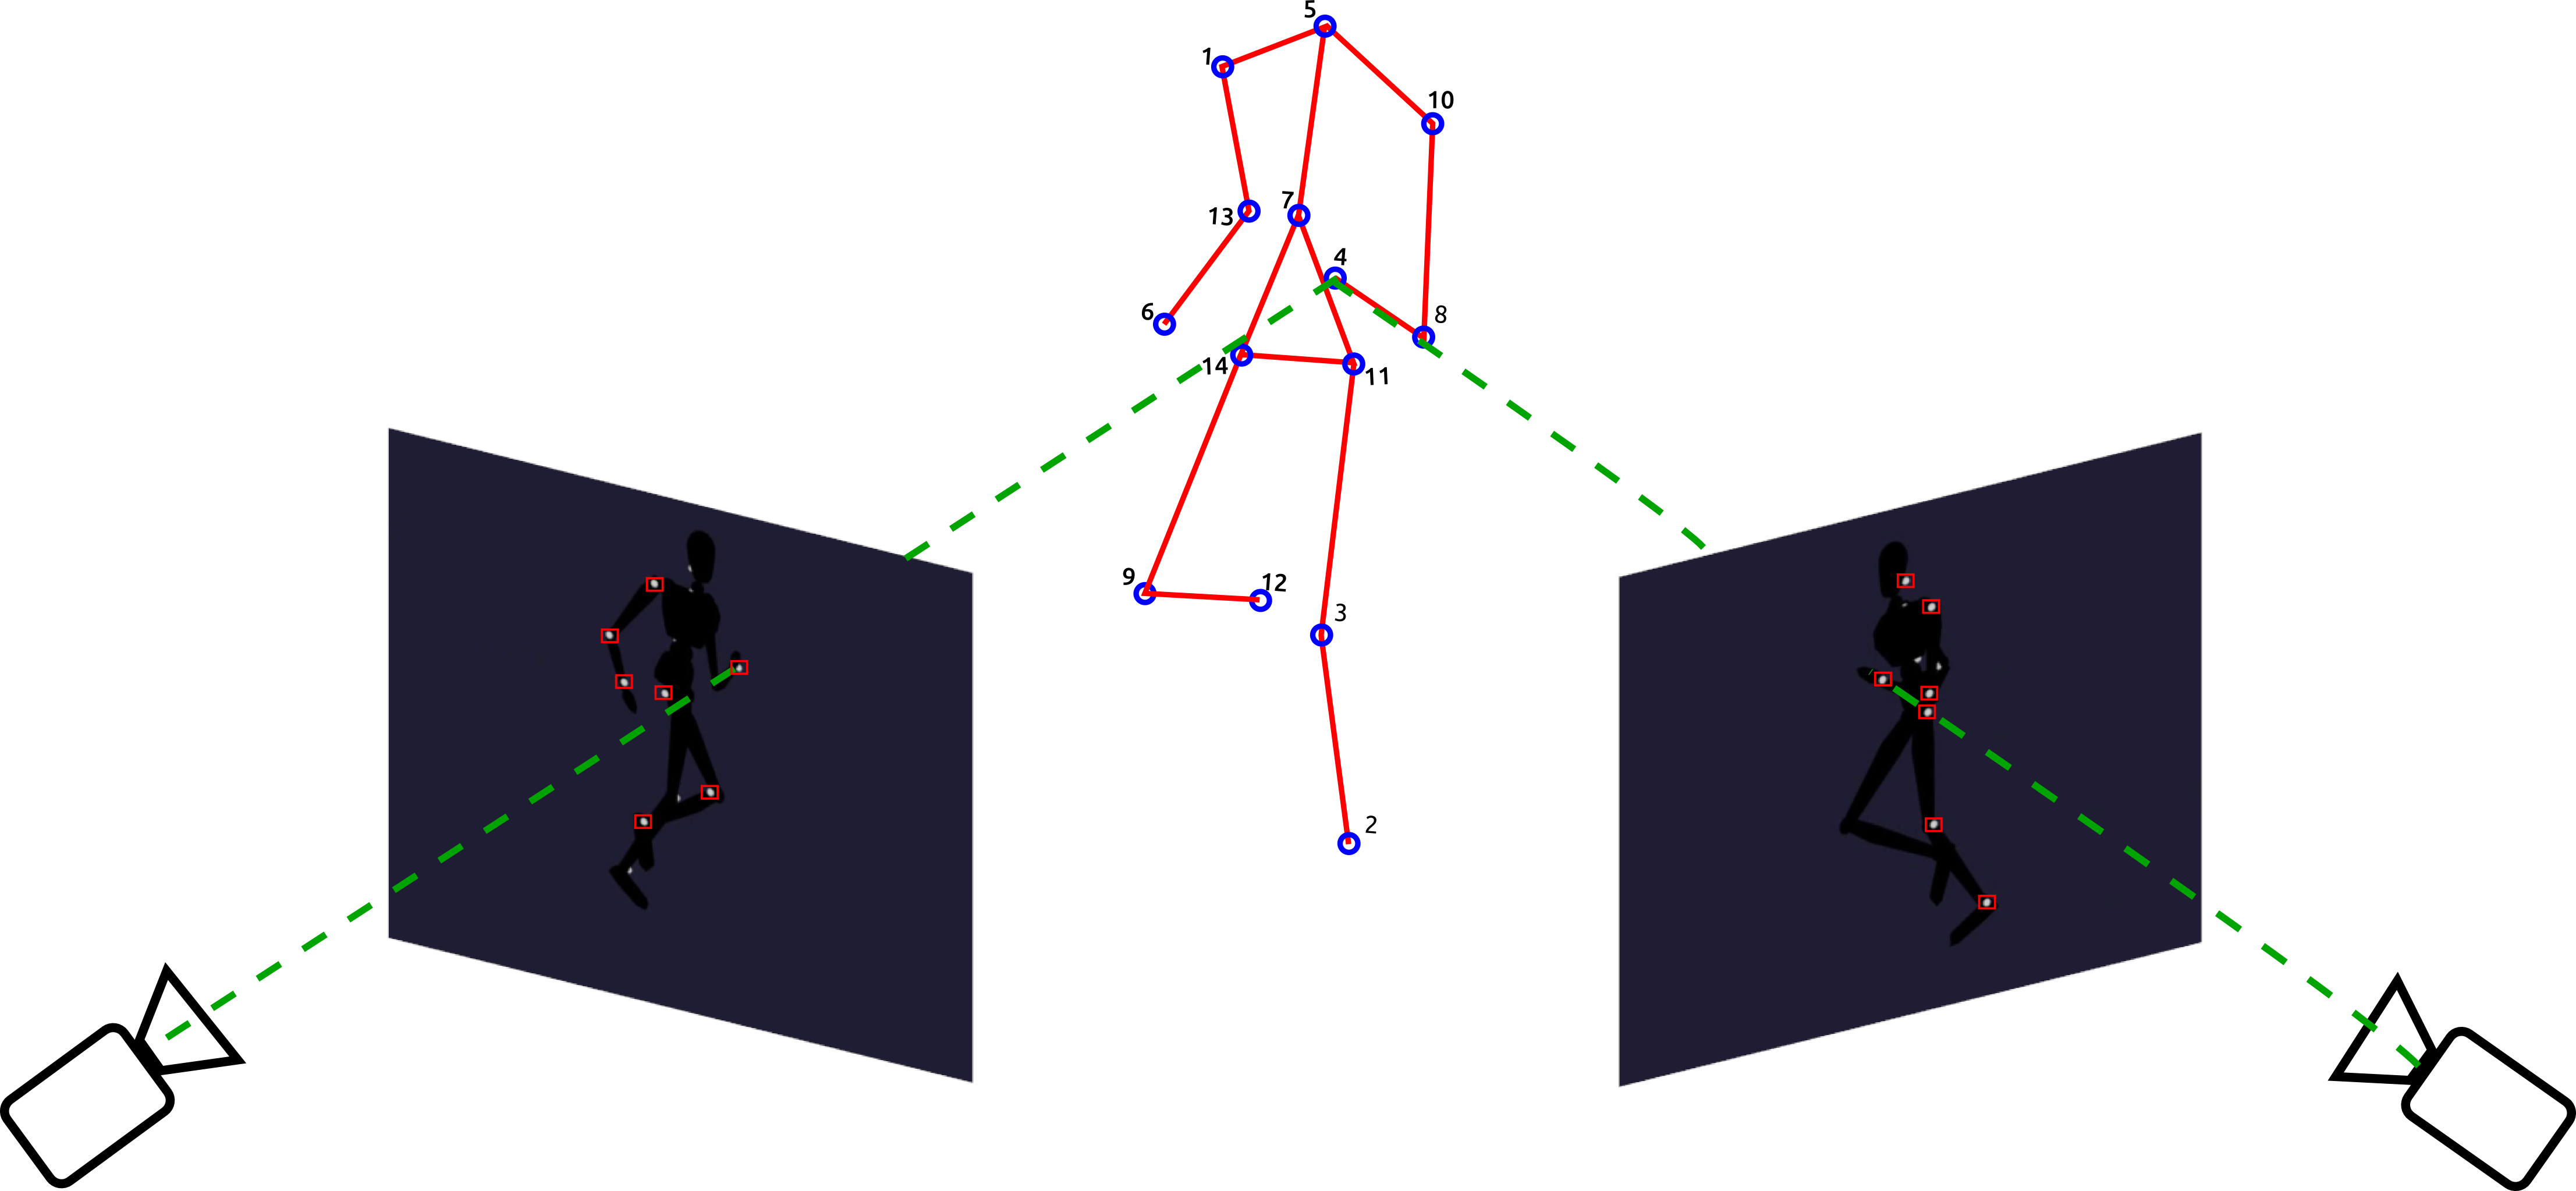
\includegraphics[scale=0.20]{img/Reconstruccion/ejemplo_reconstruccion.png}

\end{center}
\caption{Reconstruccion con dos camaras}
\label{fig: esquema_reconstruccion}
\end{figure}

%Se observa en la figura a uno de los marcadores detectados desde las dos vistas y su correspondiente punto 3D reconstruido.\\
El proceso de reconstrucción implementado consiste en tres pasos fundamentales:
\begin{enumerate}
\item Determinar aquellos marcadores detectados en las distintas cámaras que corresponden a un mismo marcador en el espacio. De esta manera se establece una correspondencia entre los marcadores detectados en las distintas vistas. Dichas asociaciones se establecen de a pares de cámaras.
\item Una vez establecidas estas correspondencias se selecciona aquella que con algún criterio pueda considerarse con mayores posibilidades de ser una asociación correcta. Luego se determina la posición en el espacio del marcador a partir de la asociación seleccionada.
\item Una vez reconstruido uno de los marcadores debe verificarse si dicho marcador fue detectado en el resto de las cámaras.
\end{enumerate}
\begin{figure}[H]
\begin{center}
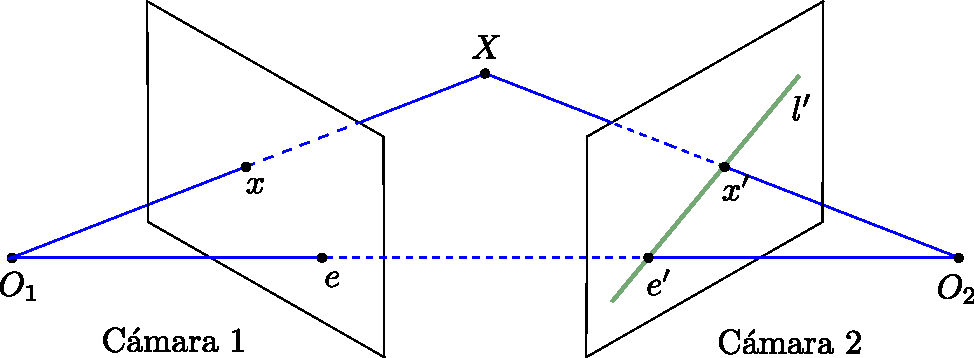
\includegraphics[scale=0.7]{img/Reconstruccion/geometria_epipolar.pdf}
\end{center}
\caption{Geometría epipolar}
\label{fig: geometria_epipolar}
\end{figure}

\subsection{Geometría epipolar}

Referencias al zisserman y al cyganek

Para explicar el algoritmo de reconstrucción es necesario describir brevemente algunos conceptos fundamentales de la geometría epipolar.  Dicha geometría es la que se presenta cuando dos cámaras en distintas posiciones se encuentran capturando el mismo espacio 3D. El análisis de esta situación permite obtener relaciones entre los puntos 3D con sus correspondientes proyecciones en las cámaras, así como las relaciones entre los propios puntos proyectados en las distintas cámaras.\\

 Como se muestra en la figura \ref{fig: geometria_epipolar}, se tiene el caso en que dos cámaras observan un mismo punto 3D en el espacio, el punto $X$. Para esto se considera el modelo \textit{pinhole} de la cámara  descrito en la sección \ref{calibracion}. En ese caso los puntos $O_1$ y $O_2$ son los centros o focos de las cámaras.\\
 
  El punto $X$ se proyecta en dichas cámaras en los puntos $x$ y $x'$. Es decir, $x$ pertenece a la intersección de la retina de la cámara 1, con la recta $\overline{O_1X}$, análogamente el punto $x'$ pertenece a la intersección de la retina de la cámara 2 con la recta $\overline{O_2X}$. A su vez, los focos de ambas cámaras $O_1$ y $O_2$ definen una recta que corta a las retinas de las cámaras en los puntos $e$ y $e'$, llamados epipolos.\\
  
  Si el punto $X$ varia sobre el espacio 3D, se tienen múltiples rectas que pasan por dicho punto y el foco de la cámara 1, el punto $O_1$. Dado que $O_1$ se proyecta en la cámara 2 como el punto $e'$ en el plano imagen, todas las rectas  $\overline{O_1X}$ se proyectan en dicha cámara como rectas que se intersectan en el punto $e'$, a estas rectas se le denominan rectas epipolares. Análogamente las rectas 3D $\overline{O_2X}$ se proyectan sobre la cámara 1 como rectas epipolares que se intersectan en el punto $e$. De esta manera se tiene que los puntos $X$, $O_1$ y $O_2$ forman un plano, llamado plano epipolar,  que intersecta a los planos imagen en las rectas epipolares.\\
  
De lo anterior se observa que si se conoce la proyección $x$ de un punto $X$ sobre una de la cámara 1, también se conoce la recta epipolar $\overline{e'x'}$ y el punto $X$ se proyecta en la cámara 2 en un punto $x'$ situado en dicha recta epipolar. Esto implica que por cada punto visto en una retina en la otra se observa como una línea.\\
 
Si los puntos $x$ y $x'$ son conocidos, sus proyecciones son también conocidas y si estos puntos corresponden a un mismo punto 3D su lineas de proyección deben intersectarse en $X$. Por lo tanto las coordenadas del punto X pueden derivarse a partir de las coordenadas de sus puntos imagen.\\
 
Para el caso de cámaras reales se tienen distorsiones de ruido, imperfecciones en las lentes de las cámaras, etc que producen que las proyecciones sean tal que el punto 3D, su proyección en la cámara y el foco de la misma no sean colineales debido a imperfecciones de las cámaras, la proyección real de un punto 3D va a ser aproximadamente el punto ideal de su proyección. \\

\subsubsection{Matriz Fundamental}

La matriz fundamental es la representación algebraica de la geometría epipolar. Si se tiene el punto $X$ y sus correspondientes proyecciones $x$ y $x'$ en las cámaras, se tiene que se verifica la siguiente condición :

\begin{equation}
(x')^T F x = 0
\label{ec: matriz fundamental}
\end{equation}
siendo  $F$ la matriz fundamental y $x$, $x'$ están en coordenadas homogéneas.\\

Si se tienen, de la cámara 1, la matriz de proyección $P$ y $x$, el punto $X$ se encuentra en la recta de proyección, que puede describirse en forma parametrica:

\begin{equation}
	X(\lambda) = P^+x+\lambda O_1
\end{equation}

donde $P^+$ es la pseudo-inversa, tal que $PP^+=I$.\
En particular se toman dos puntos de esa recta, el punto $P^+x$ ($\lambda = 0$) y el punto $O_1$ ($\lambda = \infty$).\
Si se proyectan estos puntos en la cámara 2 se obtienen los puntos $P'P^+x$ y $P'O_1$ respectivamente, siendo $P'$ la matriz de proyección de la cámara 2. Estos puntos pertenecen a la recta epipolar:

\begin{equation}
l' = (P'O_1) \times (P'P^+ x)
\end{equation}

El punto $P'O_1$ es el epipolo $e'$ de la cámara 2. Por lo tanto $l' = e' \times (P'P^+) x$, entonces se define la matriz fundamental como:

\begin{equation}
F=e' \times P'P^+
\end{equation}

Si los puntos imagen se corresponden $x \leftrightarrow x'$, entonces $x'$ se encuentra en la recta epipolar $l'=Fx$ correspondiente al punto $x$, que implica que se cumpla $0=(x')^Tl'$ y por lo tanto se verifica la condición de la ecuación \ref{ec: matriz fundamental}. Como se explicó anteriormente esto se cumple en condiciones ideales pero no para cámaras reales en las que aparecen los efectos del ruido, etc. por lo tanto debe esperase que si se tiene un punto $x$ y su correspondiente $x'$, la ecuación \ref{ec: matriz fundamental} no verifique pero en cambio de un valor próximo a cero.\\

Algunas propiedades básicas de esta matriz es que si $F$ es la matriz fundamental del par de cámaras con matrices de proyección ($P,P'$), entonces $F^T$ es la matriz fundamental del par de cámaras en sentido opuesto: ($P',P$). Por otra parte si se tiene el punto $x$ en la imagen de una cámara, su recta correspondiente recta epipolar en otra cámara es $l'=Fx$. Análogamente $l=F^Tx'$ representa la línea epipolar a x' en la segunda cámara.

\subsection{Algoritmo propuesto por Herda }

Como se explicó anteriormente, se inicia la implementación de este bloque a partir del algoritmo propuesto por Herda \cite{herda}. Este algoritmo en algunos aspectos no es descripto con el detalle suficiente tal que pueda ser replicado fielmente. Por esta razón su implementación se ha realizado tomando algunas libertades en los casos en que su interpretación pueda ser algo ambigua.\\

Por otra parte este algoritmo plantea utilizar la información del esqueleto, como por ejemplo la posición de articulaciones, distancias entre marcadores, etc.\\ (ver que el uso de información del esqueleto haya quedado bien claro en la descripción general del algoritmo).\\ Dado que este aspecto del algoritmo no fue implementado resultó necesario robustecer el proceso de reconstrucción en las partes del algoritmo donde no se utiliza esta información.\\


El algoritmo implementado por Herda utiliza la triangulación estéreo para recosntruir un punto 3D a partir de los puntos 2D detectados en las distintas vistas. La correspondencia entre distintas vistas se establece mediante la matriz fundamental, cuyos conceptos fueron explicados anteriormente. Esta matriz fundamental se obtiene mediante el proceso de calibración.\\

Los pasos que sigue el algoritmo se describen a continuación:\

\begin{itemize}
\item Se toman dos vistas y se realiza el test de la condición epipolar. Si existe una asociación no ambigua se reconstruyen  las coordenadas 3D a partir de las coordenadas 2D.

\item Las coordenadas 3D reconstruidas se reproyectan en las cámaras restantes. Los puntos 2D encontrados en esa reproyección son asociados al punto 3D. De esta forma se tiene por cada punto 3D , sus correspondientes puntos 2D asociados en las distintas vistas.\

\item Se considera que un marcador 3D está correctamente reconstruido si se reproyecta en al menos una cámara. A este tipo de reconstrucción se le llama \textit{recontrucción trinocular}.\\

\item Si el número de marcadores reconstruidos es inferior al número de marcadores que están colocados en la persona, entonces se realiza una segunda asociación entre dos vistas. En este caso la reconstrucción se realiza solamente con dos vistas.\\

\end{itemize}

Posteriormente el algoritmo plantea realizar ciertos chequeos sobre los puntos reconstruidos de manera de validarlos. Dichos chequeos utilizan información del esqueleto. Estos chequeos son de visibilidad y de oclusión.\\

Lo que se quiere verificar en dichos chequeos, es que para un determinado frame los marcadores sean efectivamente visibles por aquellas cámaras que los reconstruyeron y no están ocultos por alguna parte del cuerpo, lo que evidenciaría que las reconstrucción es incorrecta. Si esto se verifica el algoritmo busca otras vistas de las cuales reconstruir el marcador.\\

\subsection{Algoritmo implementado}

El algoritmo implementado recibe como entrada los puntos 2D de los marcadores detectados y devuelve como salida los puntos 3D reconstruidos. El primer paso consiste en establecer una asociación entre ciertos puntos 2D de distintas cámaras. Luego pasa a conjunto de bloques que se ejecutan de manera iterativa hasta que no quedan marcadores para reconstruir. En dicho bloque se busca la mejor asociación encontrada, bajo determinado criterio, luego se reconstruye un punto 3D y se realiza un proceso de validación de dicho punto. En la iteración siguiente se actualizan las asociaciones que habían sido establecidas previamente. Cuando no hay más marcadores para reconstruir se detiene el proceso iterativo y se devuelve aquellos marcadores que fueron reconstruidos en cada iteración. En la figura \ref{fig: diagrama algoritmo} se presenta un diagrama del algoritmo.\\

\begin{figure}[H]
\begin{center}
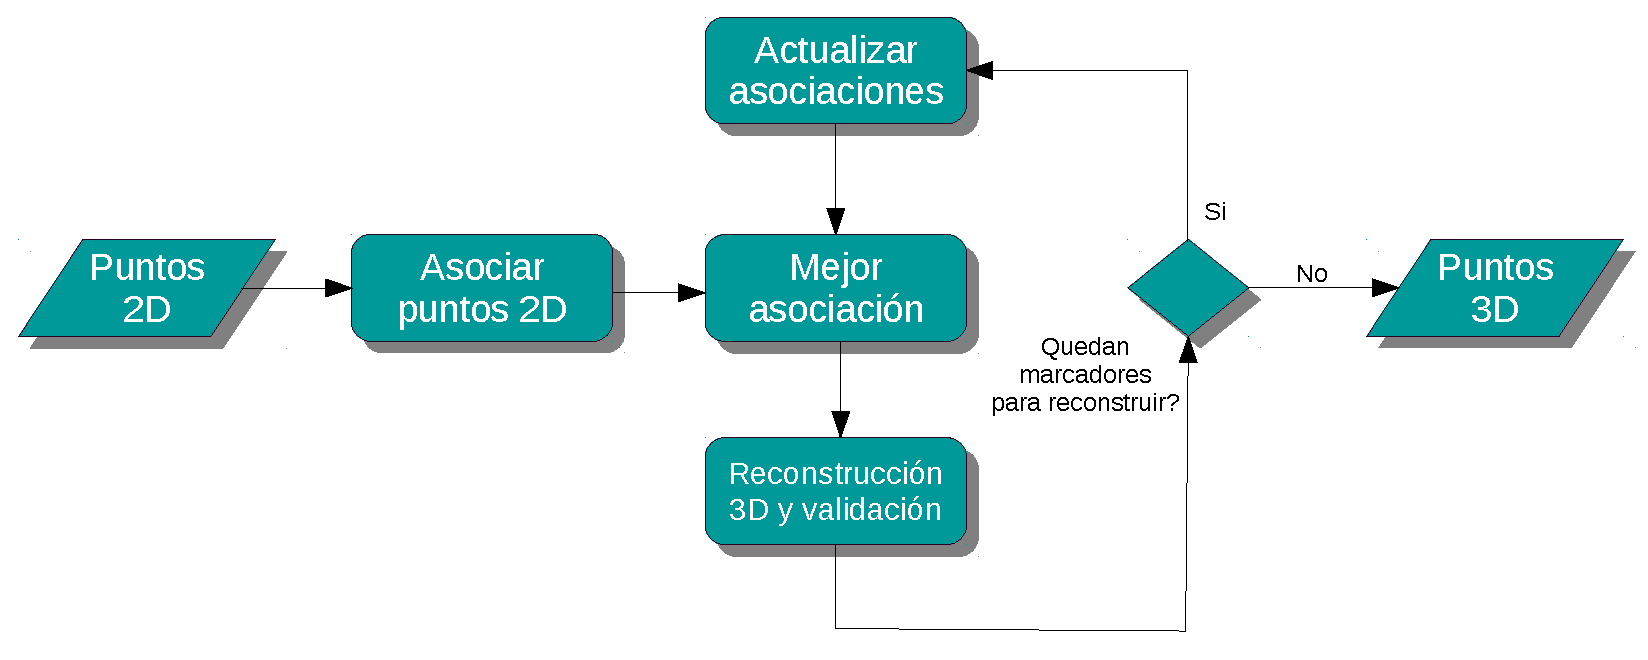
\includegraphics[scale=0.6]{img/Reconstruccion/diagrama_algoritmo.pdf}
\end{center}
\caption{Diagrama del algoritmo implementado}
\label{fig: diagrama algoritmo}
\end{figure}

A continuación se describe el funcionamiento de cada uno de los bloques:

\subsubsection*{Asociar puntos 2D}

Este bloque recibe como entrada las coordenadas de los puntos detectados en cada una de las cámaras, además de los datos de las cámaras como sus matrices de proyección. Basándose en lo explicado anteriormente el proceso puede ejemplificarse en la figura \ref{fig: cam2cam }. \\

\begin{figure}[H]
\begin{center}
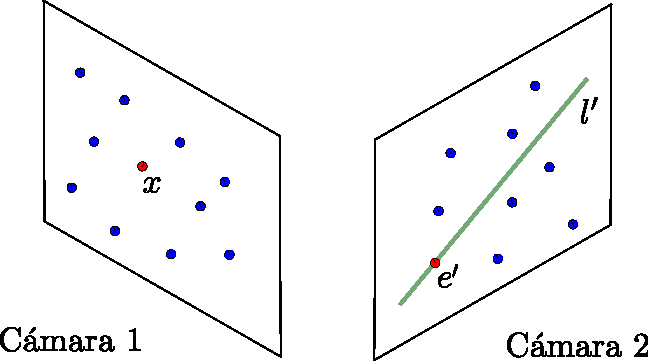
\includegraphics[scale=0.7]{img/Reconstruccion/cam2cam.pdf}
\end{center}
\caption{Asociación de puntos 2D en dos cámaras}
\label{fig: cam2cam }
\end{figure}

En primer lugar se seleccionan dos cámaras y para un punto en una de las cámaras, tomemos como ejemplo el punto $x$ de la imágen, se evalúa la ecuación \ref{ec: matriz fundamental} para cada punto en la cámara 2. Se asume que los puntos de la cámara 2 que tengan mayor posibilidad de corresponder con el punto $x$, son aquellos que al ser evaluados por la ecuación se obtengan valores próximos a cero. Esto es equivalente proyectar la recta epipolar $l'$ sobre la cámara 2 correspondiente al punto $x$ y tomar las distancias de los puntos detectados en la cámara 2 a la recta $l'$. Se demuestra que dicha distancia difiere a menos de un factor de escala respecto al valor obtenido al evaluar la ecuación \ref{ec: matriz fundamental}. De esta manera se obtiene para cada punto de la cámara 1 un conjunto de puntos de la cámara 2 ordenados según su distancia a la recta epipolar correspondiente.\\

Por lo tanto, si se seleccionan las cámaras $i$ y $j$, se consideran $N_{i}$ y $N_{j}$ el número de marcadores detectados en cada una de las cámaras respectivamente. Los marcadores detectados en dichas cámaras son los puntos de coordenadas 2D que le llamamos $m_i^r$ y $m_j^s$ para las cámaras $i$ y $j$ respectivamente\\

A su vez se realiza el mismo procedimiento a la inversa, esto es, de la cámara 2 a la cámara 1. Para cada punto de la cámara 2 se ordenan los puntos de la cámara 1 según su proximidad a la recta epipolar correspondiente a ese punto. Este procedimiento se repite para otros pares de cámaras. Respecto a la elección de los pares de cámaras se han considerado dos casos. El primero de ellos se evalúa cada cámara respecto a todas las restantes. La segunda fue considerando la disposición de las cámaras en el espacio. Ver la figura \ref{img_Laboratorio}. En ese caso se evalúa las cámaras con las que están más próximas la cámara $i$ con la cámara $i+1$. Más adelante se demuestra que este segundo procedimiento da mejores resultados. \\

\subsubsection*{Mejor asociación}

Del resultado del bloque anterior resulta necesario seleccionar aquella asociación entre puntos de dos de las vistas que tenga mayores posibilidades de correponder a la proyección en esas dos vistas de uno de los marcadores en el espacio.\\

Una de las condiciones evaluadas en un principio fue la de exigir que el marcador detectado en la cámara $i$

\begin{figure}[H]
\begin{center}
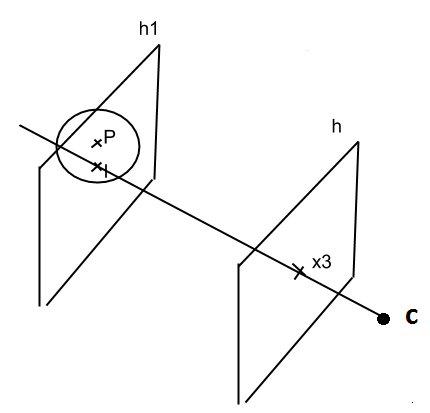
\includegraphics[scale=0.7]{img/Reconstruccion/validacion.png}
\end{center}
\caption{Geometría epipolar}
\label{fig: Etapa de validación}
\end{figure}

\subsubsection{Reconstrucción 3D y validación}


Luego de encontrar las mejores asociaciones entre dos cámaras se procede a reconstruirlas. Estas reconstrucciones deben ser validadas, para ello en principio se utiliza el  criterio propuesto por Herda \cite{herda}, se considera que una reconstrucción proveniente de dos cámaras es válida, si al proyectar sobre una tercer cámara existe al menos un punto de esta última que diste menos de un cierto valor umbral. Si efectivamente se encuentra al menos un punto, se asocia con los dos puntos que generaron la reconstrucción y se repite el proceso con el resto de las cámaras. Una vez finalizada la iteración, se retira a la pareja que genera la reconstrucción así como también a los puntos que lograron validarla, y se itera nuevamente repitiendo el proceso con la siguiente mejor pareja asociada entre dos cámaras.  


El algoritmo desarrollado si bien conceptualmente es similar, se implementa desde una óptica diferente computacionalmente más eficiente.
En lugar de llevar en cada iteración la información 3D a cada cámara, se procede a llevar la información de las cámaras una sola vez al espacio 3D y trabajar en cada iteración sobre el mismo. La información que contiene un punto en una retina se mapea en el espacio 3D sobre una recta de proyección que contiene a dicho punto y al centro de la cámara correspondiente. Supongamos que tenemos las rectas de proyección en el espacio 3D de todos los puntos contenidos en las retinas, sea $x_1$ un punto en la cámara 1 de centro $O_1$ y $x_2$ punto en la cámara 2 de centro $O_2$, como se muestra en la figura \ref{img_reconstruccion_validacion}, consideremos que $x_1$ y $x_2$ se encuentran asociados y reconstruyen al punto $X_{12}$. Idealmente $X_{12}$ se genera al interceptar las rectas de proyección de los puntos $x_1$ y $x_2$, pero debido a incertidumbres en la detección de marcadores o la calibración, comúnmente las rectas se van a cruzar. Por lo tanto la reconstrucción $X_{12}$ se genera en el punto medio del segmento perpendicular a ambas rectas.


\begin{figure}[h!]
\centering
\captionsetup{justification=centering,margin=2.8cm}
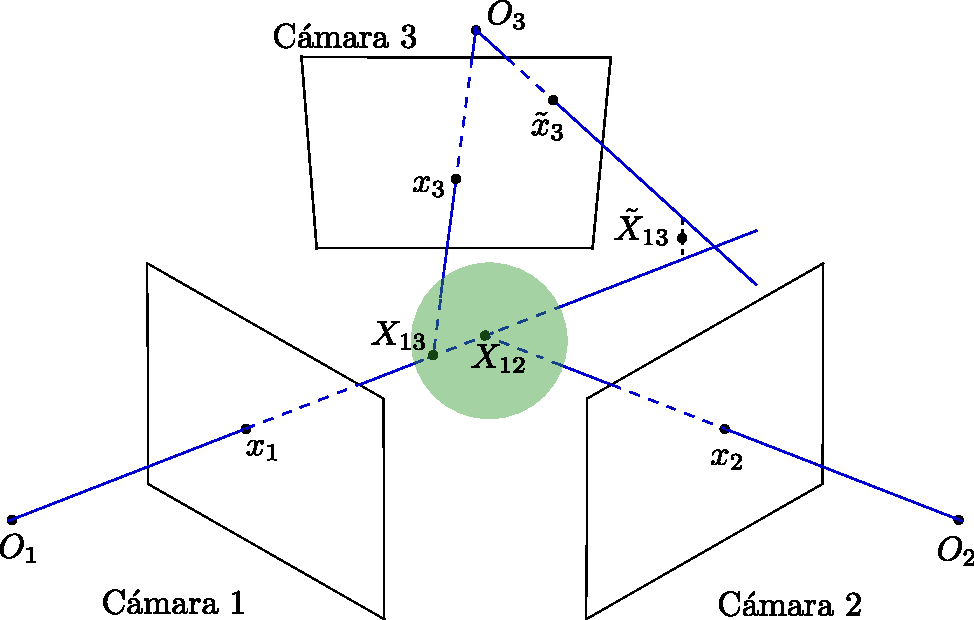
\includegraphics[scale=0.7]{img/Reconstruccion/validacion.pdf}
\caption{Reconstrucción entre cámaras 1, 2 y validación con cámara 3. \\ ~~El punto $x_3$ de la cámara 3 valida la reconstrucción.}
\label{img_reconstruccion_validacion}
\end{figure}

El algoritmo implementado asume que un punto en una cámara valida a $X_{12}$ si junto a $x_1$ reconstruye un punto 3D que se encuentra dentro de la esfera $B(X_{12}, \delta)$ de centro $X_{12}$ y radio $\delta$, donde $\delta$ es un cierto valor umbral. Notar que la elección anterior de $x_1$ sobre $x_2$ es indiferente para nuestros propósitos. Si bien este criterio difiere del postulado original, en cierta manera se considera más robusto, pues en el postulado original basta con que dos puntos en una retina se encuentran lo suficientemente cerca para obtener una validación, pero esto no implica necesariamente que provengan de puntos 3D cercanos, sin embargo bajo el nuevo criterio si dos puntos 3D se encuentran cerca, entonces es válido afirmar que sus proyecciones sobre las distintas retinas también deben estarlo. Otra ventaja es que los umbrales bajo los cuales se considera que dos puntos están "cerca'' difieren en cada una de las cámaras debido al distinto mapeo de distancias, sin embargo en el espacio 3D manejar un único umbral resulta suficiente.       


